\section{Introduction}
\label{sec:introduction}

\begin{figure}[t]
  \centering
  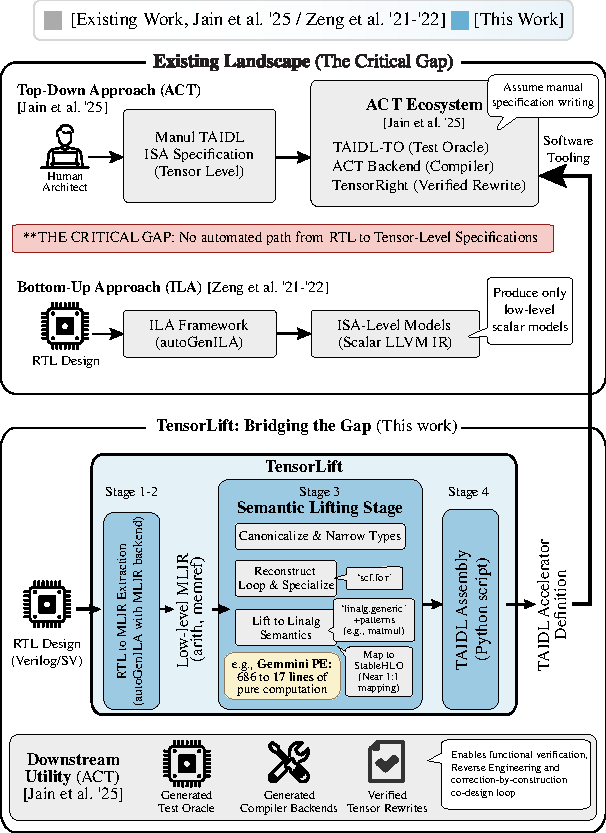
\includegraphics[width=\linewidth]{fig/overview.pdf}
  \caption{Overview of the existing landscape and TensorLift's role.
  The top-down ACT ecosystem~\cite{act-arxiv} assumes a manually written
  TAIDL specification, while the bottom-up ILA
  framework~\cite{autogeniladate, autogenilaiccad} produces only scalar-level models.
  TensorLift bridges this gap with an MLIR-based semantic lifting
  pipeline that automatically extracts tensor-level ISA semantics
  from RTL, enabling the full automated path from hardware design
  to ML framework integration.}
  \label{fig:overview}
\end{figure}

The rapid growth of deep learning workloads has driven a proliferation of specialized tensor accelerators in both academia and industry. Designs such as Gemmini, MAERI, SIGMA, Eyeriss, NVDLA, and FEATHER explore diverse microarchitectural innovations—systolic arrays, reconfigurable interconnects, flexible dataflow engines—to deliver orders-of-magnitude improvements in performance and energy efficiency over general-purpose processors. Meanwhile, a small number of platforms backed by major vendors, notably Google's TPU with XLA, Intel AMX with oneDNN, and NVIDIA GPUs with CUDA/cuDNN, enjoy mature compiler toolchains that connect them seamlessly to frameworks like PyTorch, JAX, and TensorFlow. The contrast is stark: as Table~\ref{tab:accel-landscape} summarizes, accelerators with mature, end-to-end compiler support number fewer than five, while over a dozen open-source designs lack any usable compiler backend. These accelerators can only be exercised through hand-written kernel libraries that cover a narrow set of operators and miss cross-layer fusion opportunities, leaving the vast majority of proposed hardware unable to run real ML models end-to-end.

\begin{table}[t]
  \centering
  \scriptsize
  \caption{Software stack readiness of representative open-source tensor/DNN accelerators.
  \CIRCLE{} = available, \LEFTcircle{} = partial/limited, \Circle{} = unavailable.
  \textbf{TensorLift} targets accelerators with open RTL (\CIRCLE{}/\LEFTcircle{} in col.~3)
  but missing ISA specifications (\Circle{} in col.~1).}
  \label{tab:accel-landscape}
  \setlength{\tabcolsep}{3pt}
  \begin{tabular*}{\linewidth}{@{\extracolsep{\fill}}lcccc@{}}
    \toprule
    Accelerator
      & \makecell{ISA\\Spec}
      & \makecell{Compiler\\Backend}
      & \makecell{Open\\RTL}
      & \makecell{Test\\Oracle} \\
    \midrule
    % --- No compiler backend ---
    MAERI~\cite{maeri-asplos2018}
      & \Circle      & \Circle      & \CIRCLE      & \Circle \\
    SIGMA~\cite{sigma-hpca2020}
      & \Circle      & \Circle      & \CIRCLE      & \Circle \\
    Eyeriss~\cite{eyeriss-jssc2017}
      & \Circle      & \Circle      & \LEFTcircle  & \Circle \\
    MAGNet~\cite{venkatesan2019magnet}
      & \Circle      & \Circle      & \CIRCLE      & \Circle \\
    DNNBuilder~\cite{dnnbuilder-iccad2018}
      & \Circle      & \Circle      & \CIRCLE      & \Circle \\
    FlexASR~\cite{flexasr}
      & \Circle      & \Circle      & \CIRCLE      & \Circle \\
    SPAGHETTI~\cite{spaghetti}
      & \Circle      & \Circle      & \CIRCLE      & \Circle \\
    \midrule
    % --- Partial compiler support ---
    NVDLA~\cite{nvdla}
      & \LEFTcircle  & \LEFTcircle  & \CIRCLE      & \LEFTcircle \\
    Gemmini~\cite{gemmini-dac2021}
      & \LEFTcircle  & \LEFTcircle  & \CIRCLE      & \LEFTcircle \\
    VTA~\cite{vta}
      & \LEFTcircle  & \LEFTcircle  & \CIRCLE      & \LEFTcircle \\
    DnnWeaver~\cite{dnnweaver-micro2016}
      & \Circle      & \LEFTcircle  & \CIRCLE      & \Circle \\
    \midrule
    % --- Mature (baselines) ---
    Google TPU~\cite{tpuv1}
      & \CIRCLE      & \CIRCLE      & \Circle      & \CIRCLE \\
    Intel AMX~\cite{amx}
      & \CIRCLE      & \CIRCLE      & \Circle      & \CIRCLE \\
    \bottomrule
  \end{tabular*}
\end{table}

The root cause of this software deficit lies upstream of the compiler: the ISA semantics of most accelerators have never been formally defined. In the CPU world, the ISA serves as the foundational contract between hardware and software—compilers, simulators, and verification tools are all built on top of it. For accelerators, however, ISA information is typically scattered across RTL source code, informal documentation, or exists only in the minds of hardware designers. Huang et al. formalized this observation with the Instruction-Level Abstraction (ILA), noting that the accelerator community lacks both a common framework for specifying accelerator behavior and a unified way to reason about programs that interact with accelerators. From the programming language side, Exo demonstrated that proprietary hardware interfaces force each company to maintain its own compiler fork—a cost that discourages hardware innovation and entrenches legacy platforms whose dominance stems from ecosystem lock-in rather than architectural merit. Figure~\ref{fig:overview} summarizes this landscape: the top-down ACT ecosystem assumes a hand-written TAIDL specification, while the bottom-up ILA framework produces only scalar-level models, leaving no automated path from RTL to tensor-level semantics.

Recent work has made significant strides in closing the gap from ISA specification downward. TAIDL, presented at MICRO 2025, introduced the first domain-specific language for defining tensor accelerator ISAs and showed how test oracles can be auto-generated from these definitions, achieving orders-of-magnitude speedups over hand-crafted functional simulators like Gemmini Spike. Building on TAIDL, the ACT project demonstrated that sound and complete compiler backends can be automatically generated from ISA descriptions alone, producing code that matches or outperforms hand-optimized kernel libraries. Together, these efforts establish a compelling pipeline from ISA specification to ML framework integration: given a TAIDL definition, ACT generates a compiler backend that plugs into XLA, enabling end-to-end execution from JAX or PyTorch. However, this pipeline has a critical prerequisite: someone must first write the TAIDL specification by hand—a process that requires deep understanding of the accelerator's architectural state, instruction encoding, and tensor-level semantics.

This manual specification bottleneck creates a broken pipeline in practice. On the hardware side, RTL designs iterate rapidly as architects explore microarchitectural trade-offs; on the software side, TAIDL and ACT can automate everything downstream of the ISA spec but cannot function without one. The result is that building compiler and simulator support still involves considerable manual effort, slowing innovation and widening the gap between hardware and software research communities. The 3LA methodology corroborates this assessment: even with the ILA formal framework available, testing prototype accelerator designs on real applications end-to-end remains prohibitively difficult due to the cost of constructing specialized compiler and simulator support. This bottleneck also limits the potential of emerging LLM-based agents for EDA, which are poised to transform hardware design workflows but require machine-readable hardware semantics as input—semantics that, for most accelerators, simply do not exist in any structured form.

In this paper, we present TensorLift, the first approach to automatically extract tensor-level ISA semantics from accelerator RTL. TensorLift employs an MLIR-based semantic lifting pipeline consisting of seven progressive passes that transform low-level CIRCT/FIRRTL representations into high-level tensor operations, bridging the abstraction gap between gate-level hardware and the ISA-level semantics required by tools like TAIDL and ACT. We evaluate TensorLift on the Gemmini accelerator, achieving 100\% instruction coverage by extracting all 11 hardware instructions. Our analysis also reveals that 4 of the 15 entries in TAIDL's Gemmini specification—softmax, GELU, layernorm, and fused add-with-transpose—are in fact software-composed macro-instruction sequences rather than hardware ISA primitives, a distinction that TensorLift's bottom-up extraction naturally surfaces. By filling the frontmost gap in the RTL-to-framework pipeline, TensorLift enables a fully automated path from RTL to ML framework integration, as illustrated in Figure~\ref{fig:overview}. The complete pipeline---RTL through TensorLift to ISA specification, then through ACT to a compiler backend plugged into XLA---requires no manual specification effort at any stage.

In summary, this paper makes the following contributions:

\begin{itemize}
\item We propose the first method for automatically extracting tensor-level ISA semantics from accelerator RTL, eliminating the manual specification bottleneck that currently blocks the adoption of automated compiler generation tools.
\item We design a 8-pass MLIR-based semantic lifting pipeline that progressively abstracts from CIRCT/FIRRTL through control flow recovery, memory access pattern analysis, and datapath semantics extraction to tensor-level operation identification.
\item We evaluate TensorLift on the Gemmini accelerator, demonstrating 100\% hardware instruction coverage (11/11) and identifying the boundary between true hardware ISA and software-composed macro-instructions.
\item We complete the end-to-end automated pipeline from RTL to ML framework, enabling agile software stack construction that can keep pace with hardware design iteration.
\end{itemize}




